\Chapter{Természetes nyelvfeldolgozás}

\Section{Történeti áttekintés}

Az emberi nyelv egy komplex médium gondolatok, információk, ötletek és érzelmek átadására, továbbítására. Nagyon nehéz ezt a működést matematikai formulákkal, képletekkel leírni. A legegyszerűbb mondatok leírása is több oldalas feladat lehet formális nyelveket használva. Emiatt különösen nehéz dolguk van a gépeknek az emberi nyelvek értelmezésével, vagyis a természetes nyelvfeldolgozással(NLP - Natural Language Processing).

Az "fordító gép" fogalom első előfordulása az 1930-as évek közepére tehető. Akkoriban két szabadalom is létezett a technológiára. Az első szabadalom \textbf{Georges Artsrouni} nevéhez köthető, aki egy kétnyelvű szótárat használt arra, hogy átfordítsa a szavakat közvetlenül egyik nyelvről a másikra egy papírszalag segítségével. Ez egy nagyon kezdetleges megoldás volt, mivel a nyelvtani különbségekkel nem tudott mit kezdeni. A második egy orosz szabadalom volt \textbf{Peter Troyanskii} nevéhez fűződően. Ő szintén egy kétnyelvű szótár felhasználásával próbált fordítani, azonban ő figyelembe vette az egyes nyelvtani szabályokat is. Mindkét megközelítés hasznosnak bizonyult technikai szempontból, azonban működő modellt nem igazán sikerült készíteniük, inkább koncepcionális megoldások voltak.\cite{history}

Az első kísérlet az NLP alkalmazására a németekhez köthető a 2. világháború alatt. Ők fejlesztették ki az \textbf{Enigma} nevű gépezetet, melyet titkos üzenetek kódolására használtak. A gép képes volt kódolni, illetve továbbítani az egyes parancsnokoknak és katonai egységeknek szánt üzeneteket. Később erre válaszul az angolok elkészítették a \textbf{Colossus} nevű gépet, amely képes volt dekódolni az Enigma által kódolt üzeneteket, így járulva hozzá a szövetségesek későbbi győzelméhez.
A második világháború alatt az angolok kriptográfiai kutatásai elsősorban a Bletchley Park-ban zajlódtak. Itt dolgozott Alan Turing is kollégáival, akihez később számos új megközelítés is kötődik az informatika történetében.\cite{history}

\begin{figure}[h]
\centering
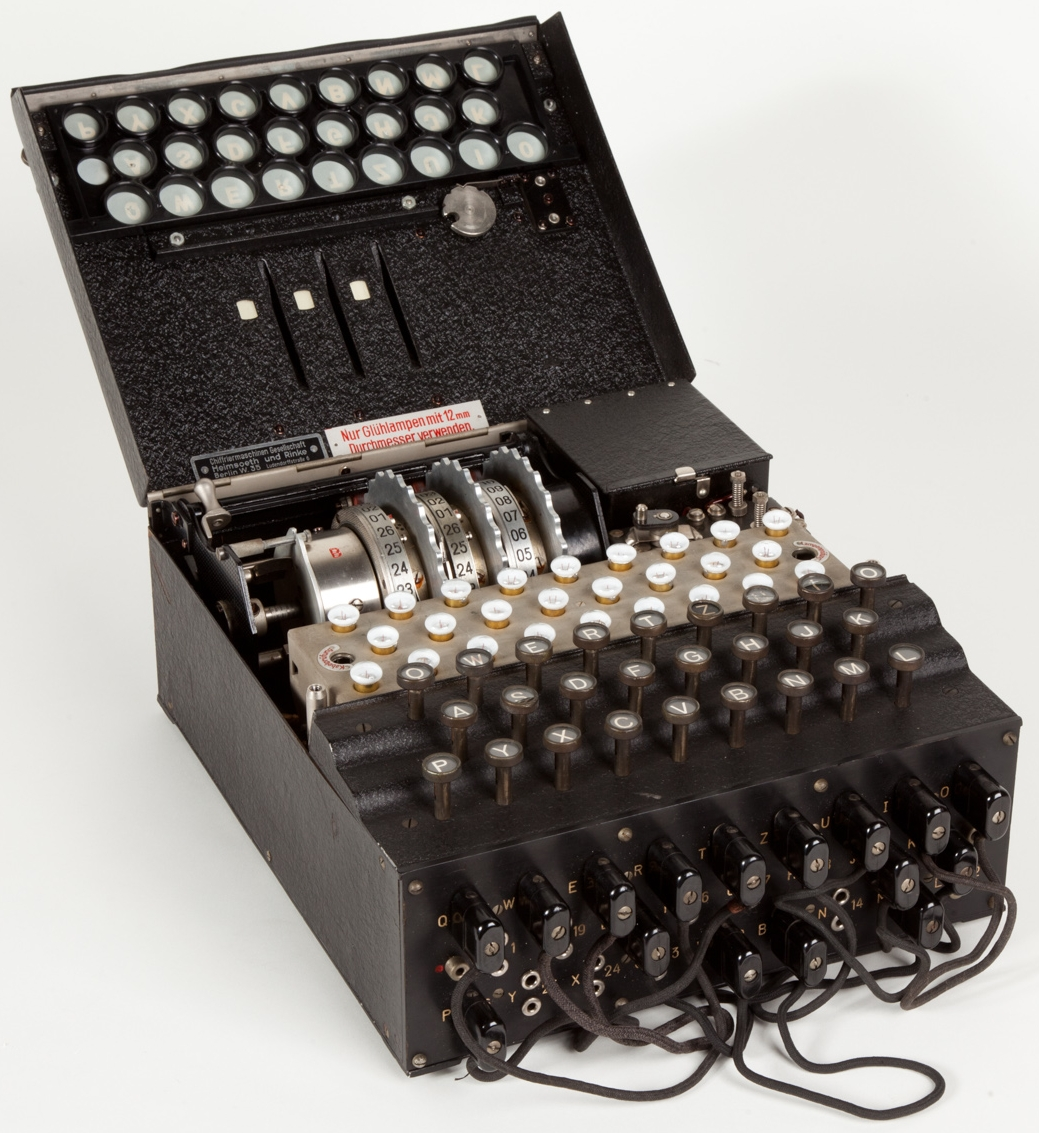
\includegraphics[scale=0.6]{images/enigma.jpg}
\caption{Az Enigma 1-es modell \cite{enigma}}
\label{fig:enigma}
\end{figure}

1950-ben \textbf{Alan Turing} megalkotta a Turing-tesztet, ami úttörővé vált a természetes nyelvfeldolgozás területén. A teszt lényege, hogy eldöntse egy gépről tud-e emberhez hasonlóan gondolkodni. Magához a teszthez 3 személyre van szükség: 1 férfira, 1 nőre és 1 kérdezőre. A kérdezőt elszeparálják a játékosoktól. A teszt során a kérdező megpróbálja meghatározni a másik két személy nemét kérdések és rájuk adott válaszok által írásban. A csavar a tesztben, hogy az egyik személy a helyes megoldás felé próbálja terelni a kérdezőt, míg a másik próbálja átverni őt és a helytelen megoldás felé vezetni. Turing azt javasolta, hogy ezt a játékost cseréljék le egy gépre. Ha a kérdező sikeresen meg tudja határozni mindkét játékos nemét, akkor a gép elbukott a Turing-teszten, egyébként pedig átment rajta. Maga a teszt nem szimplán arról szól, hogy a gép meg tudja-e oldani ezt a problémát, hanem hogy eldöntse tud-e olyan feladatokat végezni a gép, amit csak egy ember tud, vagyis hogy képes-e emberként gondolkodni.

Ahhoz, hogy a gépek képesek legyenek megérteni az emberi nyelveket elengedhetetlen a megfelelő nyelvtanok alkalmazása. Az egyes mondatok értelmezéséhez a gépnek ismernie kell a különböző nyelvtani szabályokat, vagyis tudnia kell, hogy például vannak-e ragok az adott nyelvben, milyen igék, tárgyak vannak, illetve ismernie kell a különböző mondathatároló karakterek jelentéseit. 1957-ben \textbf{Noam Chomsky} könyvében\cite{chomsky} bevezette a szintaktikai szerkezetek fogalmát. Munkájában nagy hangsúlyt fektetett a nyelvi szerkezetek formalizálására. A természetes nyelveket is el tudta helyezni egy hierarchiában, melynek köszönhetően elkezdődhetett az NLP feladatok gépeken történő megvalósítása. A későbbiekben Charles Hockett számos hátrányt fedezett fel Chomsky megközelítésében, mivel az egy jól meghatározott és stabil struktúrát és formális rendszert tételezett fel a nyelvek mögött, ami az emberi nyelvekre csak kivételes esetekben volt igaz.

Az NLP-t legelőször a gépi fordításban használták. A gépi fordítás lényege, hogy olyan programokat készítsünk, melyek képesek egyik emberi nyelven írt szövegről egy másik emberi nyelven írt szövegre fordítani, akár valós időben is. Ilyen fordító volt 1954-ben a \textbf{Georgetowni Egyetem} és az \textbf{IBM} által közösen fejlesztett program\cite{ibm_trans} is, ami 60 orosz nyelvű mondatot is képes volt angolra fordítani. Működése egyszerű volt: szótár használatával közvetlenül fordította a mondatokat egyik nyelvről a másikra. Ezt a szótárat pedig a program készítői felügyelték és tartották karban. A készítők nagy elvárásokat támasztottak programjuk felé, azonban financiális okok miatt végül abba kellett hagyniuk a projektet.

1960-ban \textbf{Terry Winograd} elkészítette \textbf{SHRDLU} nevű programját\cite{history}, ami egyike volt az első NLP-t használó programoknak. A programnak lehetett különböző utasításokat adni, hogy nevezzen meg objektumokat egy képen, mozgasson alakzatokat, illetve le lehetett benne kérdezni az aktuális állapotot a blokkokból álló virtuális világában. A szoftver lenyűgözte a mesterséges intelligenciával foglalkozó szakembereket és számos új megoldást inspirált, azonban komplexebb, valós világból származó problémák megoldására nem igazán lehetett használni.

\begin{figure}[h]
\centering
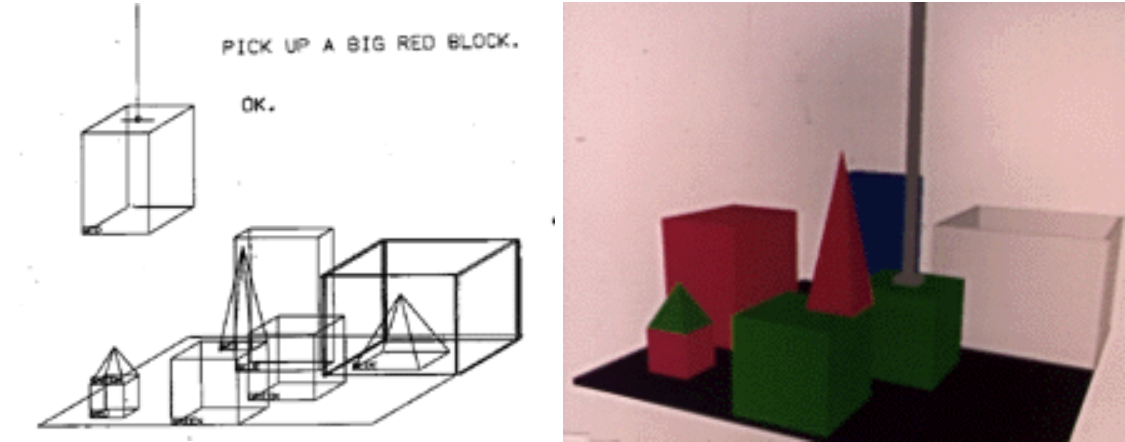
\includegraphics[scale=0.5]{images/shrdlu.png}
\caption{Az SHRDLU grafikus felülete. Bal oldalon az eredeti, jobb oldalon a később színezett változat. \cite{shrdlu}}
\label{fig:shrdlu}
\end{figure}

1969-ben \textbf{Roger Schank} bevezette a tokenek használatát a természetes \\
nyelvfeldolgozásban.\cite{history} Az egyes tokenek különböző valós világbeli objektumokat, cselekvéseket, helyeket és időt jelöltek. Ezen tokenek segítségével a gép könnyebben megtudta érteni az egyes mondatok jelentéseit. Ez a tokenes megoldás a mai napig használatban van és részben példaprogramunkban is használni fogjuk.

Az eddigi felvázolt megoldások mindegyike nyelvtani szabályok és struktúrák alapján próbálta értelmeztetni a géppel a mondatokat, azonban tudjuk, hogy pusztán ezek ismerete nem elég egy adott mondat helyes feldolgozásához. Pontosan emiatt 1970-ben \textbf{William Woods} bevezette az ún. kiterjesztett átmeneti hálózatokat(\textbf{ATN}) a természetes nyelvek reprezentációja során.\cite{atn} Működésének lényege, hogy az elérhető információk felhasználásával véges automatákat használt rekurzióval a mondatok értelmezéséhez. Tehát a program ad egy lehetséges megoldást az adott szöveg jelentésére és ahogy egyre több információt adunk meg úgy kezdi el javítani, finomhangolni a jelentést is. Amíg nem biztosítunk elég információt a hálózat számára, addig rekurzióval próbál megoldást találni vagy képtelenné válik biztos jelentés meghatározására. Ez a rekurzió szerű működés megfigyelhető napjaink szöveggeneráló és chatbot alkalmazásaiban is.

A közelmúltban új trendek kezdtek el megjelenni az NLP területén. A korábbi szigorú kézi szabályhalmazokat alkalmazó megoldásokat elkezdték háttérbe szorítani a különböző \textbf{gépi tanulást} használó valószínűségeken alapuló algoritmusok, melyek első jelentősebb felfutása az 1980-as évekre tehető. Ilyen algoritmusok voltak például a döntési fák, melyek ha-akkor szabályok alkalmazásával képesek voltak optimalizálni az egyes NLP feladatok eredményeit.

Napjainkban a figyelem elsősorban a \textbf{mély tanulást} alkalmazó megoldások felé irányult, ami nem is lehet véletlen, hiszen ezek a megoldások a neurális hálózatok használatával az ember információfeldolgozó képességét próbálják lemásolni és gépekre átültetni. Ezen megoldások lényege, hogy ne próbáljunk meg fix szabályokat vagy formulákat megadni a gépnek egy szöveg értelmezésénél, hanem mutassunk példákat a különböző nyelvi elemekre és alakítsa ki a gép magának ezeket a szabályokat és összefüggéseket. Mindezen változtatásokra a probléma megközelítésében azért volt szükség, mert a természetes nyelvfeldolgozás során számos olyan nehézséggel találkozhatunk, melyek más formálisabb, kötöttebb területeken egyszerűen nem jelennek meg. Ezen problémaköröket fogom ismertetni a következő alfejezetben.

\newpage

\begin{figure}[h]
\centering
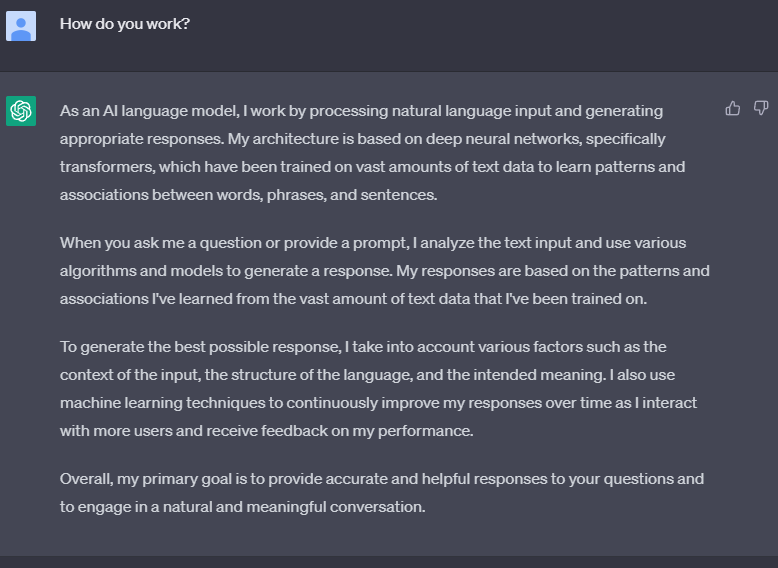
\includegraphics[scale=0.6]{images/chatgpt.png}
\caption{Beszélgetésrészlet a ChatGPT nevű intelligens chatbot-tal.}
\label{fig:chatgpt}
\end{figure}

\Section{A természetes nyelvfeldolgozás nehézségei}

Mint minden szakterületnek, így a természetes nyelvfeldolgozásnak is vannak nehézségei vagy akár adott technológiával pillanatnyilag megoldhatatlan feladatai. Maguknak a természetes nyelveknek a gépek általi megértése is ilyen megoldhatatlannak gondolt probléma volt a 20. században, hiszen talán ez az az utolsó válaszvonal az emberek és a gépek között, melyet átlépve már a technológiai szingularitás küszöbére kerül az emberiség. Továbbá ez az a szakasz, ahol teljesen egyértelműen meg tudunk különböztetni egy emberi és egy gépi agyat. De melyek is azok az egyes problémakörök, melyek alapján jogosan gondolhatnánk lehetetlennek a gépek számára az emberi nyelvek megértését?

Az első ilyen nehézség az a \textbf{többértelműség}. Bizonyos szavak szándékos vagy nem szándékos módon többféle jelentéssel is bírhatnak számunkra. Ez adódhat abból, hogy egy adott szó átvételre került egy másik nyelvből és ütközik egy már meglévő, de más szófajú szóval. Ilyen például a "vár" szavunk, amit használhatunk igeként és főnévként is. Ebben az esetben nem szándékos többértelműségről beszélünk. De akadhat olyan eset is például a szépirodalomban, ahol igenis direkt módon van használva a többértelműség. Ilyen alkalmazását találhatjuk meg például Kosztolányi Dezső \textit{Aranysárkány} című művében, ahol a mű központi alakja Novák Antal vitatkozik, hogy mit jelent a diákok által készített magasban repülő sárkány. Novák játéknak gondolja, míg Fóris fenyegető hatásúnak. Nézetkülönbségük a "sárkány" szó kétértelműségén alapul, ami jelenthet reptetésre való papírsárkányt és ősi mítoszokból eredő tűzokádó teremtményt is. Ez a példa egyben a műfordítás egyik problémáját is felveti, hiszen, ha ezt a szöveget angol nyelvre szeretnénk átfordítani, akkor bajban lennénk, hiszen az angol nyelvben külön szó létezik a papírsárkányra(kite) és az állati sárkányra(dragon), így nem lenne értelmezhető a két szereplő vitája.

Láthatjuk, hogy számos nehézség következik a kétértelműségből és így, ha NLP-vel foglalkozunk, akkor kezdenünk is kell vele valamit. De hogyan tudnánk megoldani, hogy a gép el tudja kerülni ezt a problémát és helyesen értelmezzen szépirodalmi szövegeket? 
Vegyük példának ezt a mondatot:

\vspace{0.5cm}
\centerline{\textit{,,A szolgáltatónak kell fizetni.''}}
\vspace{0.5cm}

\noindent Ez a mondat 2 különböző jelentést is takarhat:

\begin{itemize}
\item Valakinek be kell fizetnie egy bizonyos díjat egy szolgáltatónak.
\item Magának a szolgáltatónak kell kifizetnie egy adott összeget valakinek.
\end{itemize}

Mind a 2 értelmezés helyes szintaktikailag, azonban szemantikailag nem mindegy, hogy hogyan értelmezzük. Természetesen a mondat pontos jelentése egyértelművé válik, amint megismerjük a kontextust  melyben a mondat elhangzott, de mindehhez komplex háttértudásra van szükségünk. Ennek a háttértudásnak az ismerete hiányzott eddig a különböző NLP feladatok megoldására írt programokból, hiszen ezek rengeteg adatot, metaadatot, szabályt és egyéb heurisztikát igényelnek. Mi emberek az evolúció, illetve az egyéni fejlődés során gyerekkortól megismertük ezt a szükséges háttértudást egy ilyen mondat értelmezéséhez, viszont a gépek nem rendelkeztek eddig az ezekhez szükséges eszköztárakkal. Tehát a megoldás, hogy valamilyen módon példákat kell mutatnunk a gépnek ezekre az esetekre és tanítanunk kell folyamatosan, hogy el tudja dönteni a kontextus alapján ezen szövegek jelentését.

Egy további nehézség lehet a természetes nyelvfelismerésben az \textbf{apró részletek} és a \textbf{szórend} okozta különbségek az értelmezésben. Sokszor egyetlen szó, de akár egy betű vagy írásjel is teljesen megváltoztathatja egy mondat jelentését. Tekintsük mondjuk ezeket a példákat:

\vspace{0.5cm}
\centerline{\textit{,,Lőttem egy gyönyörű fotót.''}}
\centerline{\textit{,,Lőttem egy gyönyörű vadat.''}}
\vspace{0.5cm}

Amellett, hogy a "lőttem" szó többértelmű és ez önmagában is okozhat problémákat vegyük észre, hogy a két mondat csupán egyetlen szóban különbözik. Ebben az esetben, ha például egy korábbi megoldással egy koszinusz hasonlósági számítással szeretnénk értelmeztetni a géppel ezt a mondatot és el szeretnénk helyezni a mondatok egy bizonyos csoportjában akkor ez a két mondat jelentését tekintve nagyon közel kerülne egymáshoz. Tehát a gép számára bizonyos hibahatárok között ugyanazt jelentené a két mondat, annak ellenére, hogy két teljesen más jelentésről van szó. Mindezek miatt szükségessé vált, hogy a gépet folyamatosan tanítsuk újabb példákkal, hiszen maga a nyelv is folyamatosan fejlődik. Korábban a "lőttem" szó tényleges lövést jelentett, ma pedig már egy fotó elkészítését is jelentheti. Tehát egy olyan mechanizmusra van szükségünk, amit nem elég egyszer elkészítenünk vagy betanítanunk, hanem rendszeresen frissíteni kell a tudását az idők során.

Újabb problémákat vetnek fel a szépirodalomban megtalálható \textbf{költői képek}, mint a metafora, az allegória, a metonímia vagy a különböző szimbólumok értelmezése. Ezek értő használata még az emberek között is a legmagasabb kulturális szintnek felel meg, így ezeket a gép se fogja egyszerűen megérteni és használni. Ez a problémakör ráadásul nem csak a természetes nyelvfelismerést érinti, hanem például a  képfeldolgozást is. Ugyanis ezek a művészeti eszközök megjelenhetnek a szobrászatban vagy a festészetben is. Számos példa volt már a gyakorlati felhasználásában ezeknek a képfelismerő algoritmusoknak, ahol mondjuk meztelenséget kellett volna az algoritmusnak kiszűrnie egy adott képen, azonban olyan képeket is szimplán meztelenségnek kezdett el érzékelni, ahol egy szobor vagy egy festmény, egy művészeti alkotás volt látható. Itt a gép láthatóan nem volt képes a meztelenségnek, mint alkotói eszköznek, a szabadság, az újjászületés vagy a tisztaság szimbólumának a megértésére. Ugyanez igaz a szövegfeldolgozásra is, ahol például egy szimpla szó, mint a "tenger" Petőfi Sándor \textit{Föltámadott a tenger} című versében egyszerre jelenti a valódi nagy kiterjedésű víztömeget, illetve a népek tömegét. Viszont a gép nem tudja jelenleg ezt a komplex kapcsolatot feltárni a nép és a tenger között akármennyi példát is mutatunk rá neki. Ez a kapcsolat akkor is egy hosszú megértési folyamatnak lesz az eredménye, mely magába foglal történelmi, művészeti, nyelvi és érzelmi tudást.

\newpage

\begin{figure}[h]
\centering
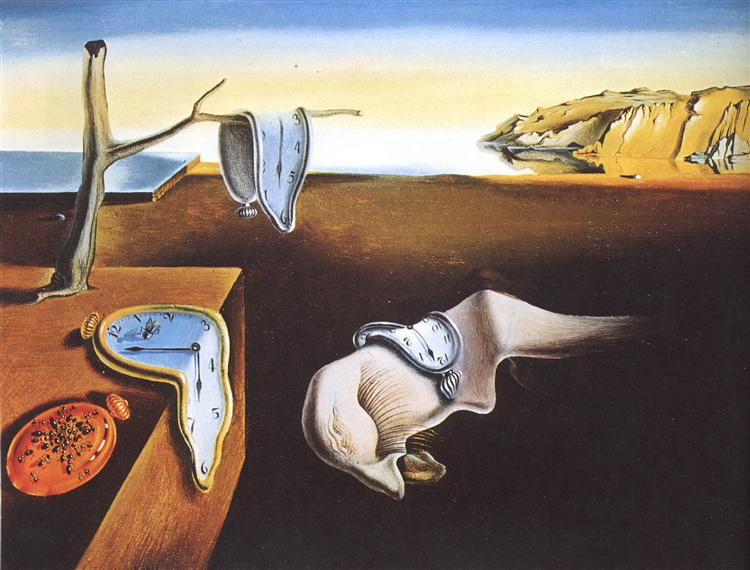
\includegraphics[scale=0.5]{images/metaphor.jpg}
\caption{Salvador Dalí Az emlékezet állandósága című szürrealista festménye, melyen az olvadt órák az időnek, az idő folyásának, relativitásának a metaforái.}
\label{fig:metaphor}
\end{figure}

Az \textbf{irónia} és a \textbf{szarkazmus} is számos félreértés tárgya lehet a különböző NLP algoritmusoknak, de akár még egyes emberi moderátoroknak is. A két fogalmat gyakran keverik, illetve mossák össze, és bár valóban van közös metszetük, de alapvetően eltér a jelentésük. Az irónia azt jelenti, hogy a szöveg szó szerinti értelme és a tényleges, a beszélő szándéka szerinti értelme ellentétes. Itt már rögtön találkozunk egy NLP szempontjából elsőre nehezen értelmezhető fogalommal a "szó szerinti" jelentéssel. Ez a probléma a gép számára jelentős kihívást jelent, hiszen ha adunk a gépnek egy mondatot és megkérdezzük tőle a jelentését, akkor a gép elsőre helyesnek tűnően fogja megválaszolni nekünk a jelentést, azonban mi tudni fogjuk, hogy ez a jelentés nem pontos. A szarkazmus ezzel szemben csak annyit jelent, hogy a beszélő szándéka egy adott kifejezéssel, hogy gúnyoljon valakit vagy valamit vicctől és humortól mentesen, de mégis a sorok között elbújtatott formában. Tehát a gépnek nem elég egyetlen jelentést számon tartania az egyes mondatokról és kifejezésekről, hanem tudnia kell az összes lehetséges jelentését az adott szövegnek. Vegyük például a következő mondatot:

\vspace{0.5cm}
\centerline{\textit{,,Na jól állunk!''}}
\vspace{0.5cm}

Ennek első jelentése, hogy jól haladnak a dolgok, tehát valami pozitív történt vagy történik. Második, valódi jelentése azonban pont ellentétes, tehát rosszul állnak a dolgok, negatív a kontextus. Ez az ellentét a gép szempontjából értelmezhetetlennek tűnik, azonban itt is, akár csak a többi nehézség esetében a kontextusok megtanulása megoldhatja ezen problémákat.

Utolsó fontosabb problémakörünk a különböző \textbf{szöveghibák}, illetve az egyes nyelveket érintő \textbf{forráshiány}. Az írott, illetve diktált szövegekben gyakoriak az elírások és a helytelenül használt szavak. Ezek egyértelműen megváltoztatják vagy egyenesen értelmezhetetlenné teszik a szövegek feldolgozását. Ezen hibák oka lehet a figyelmetlenség, az akcentus vagy az esetleges dadogás. Ilyenkor használhatunk különböző nyelvtani javítóprogramokat a bemeneti szövegeken, azonban itt se garantált a tökéletes működés. Ez a probléma is rámutat arra, hogy egy ilyen NLP feladatot megoldó programnak több különböző problémacsoportot kell tudnia kezelni és nem elég szimplán szövegeket megtanulnia.

A másik probléma, ami engem is érintett diplomamunkám gyakorlati része során az a szöveges forráshiány bizonyos nyelveken. Ahhoz, hogy az NLP feladatokat megvalósító modern alkalmazásaink megfelelően működjenek elengedhetetlen, hogy az adott nyelveken jól szűrt és kedvezően formázott szöveges forrásaink vagy bemeneteink legyenek. Ez azért fontos, mert később a program a tudásbázisát ez alapján a bemenet alapján fogja felépíteni és a fentebb felsorolt problémákat is ez alapján kell majd neki felismernie és megoldania. Például ahhoz, hogy angol nyelven tudjunk kérdéseket generáltatni egy programmal, ahhoz szükség lehet egy olyan angol nyelvű szöveges forrásra, ahol adott egy témakör és egy szöveges kontextus, valamint adottak hozzá illő kérdések. Ha ez nem áll rendelkezésünkre, akkor máris egy hatalmas problémával találjuk szembe magunkat, hiszen nem fogunk tudni alkalmas példákat mutatni a programunknak az adott feladat megvalósításához, illetve a tesztelést is meg fogja nehezíteni.

\Section{NLP feladatok}

Mivel az emberi agy digitális újraalkotása egy meglehetősen nehéz és bonyolult feladat, így a különböző csak emberek által elvégezhetőnek vélt NLP feladatokat külön-külön csoportokba és alcsoportokba szokták bontani. Természetesen a jövőben elkészülhet egy olyan mesterséges intelligencia, ami már egyben képes lesz az összes NLP feladat elvégzésére, de egyelőre itt még nem, vagy csak részben tartunk.

Az első fontosabb NLP terület az a \textbf{szintaktikai elemzés}. Ennek során az algoritmusnak azonosítania kell az adott szöveg szintaktikai struktúráját és fel kell tárnia az egyes szavak és mondatok függőségi relációját. Ezen folyamat eredménye lehet például  egy ún. elemzési fa, mely egy rendezett és gyökérelemmel rendelkező fa-struktúra, amelyről leolvasható lesz az adott szöveg szintaktikai struktúrája valamilyen kontextusfüggetlen nyelvtan szerint. Ezen feladat eredményeit fel lehet használni az információkinyerés, gépi fordítás, illetve a nyelvtani ellenőrzés, javítás területén.

Egy másik NLP terület a \textbf{szemantikai elemzés}, mely már az adott szöveg tényleges jelentésére fókuszál. A fentebb felsorolt NLP problémák miatt talán ez a feladat tekinthető a legnehezebbnek. A szemantikai elemzéshez kapcsolódó feladatok során elemezzük a mondatok struktúráját, az egyes szavak között lévő interakciókat és a kapcsolódó fogalmakat, annak érdekében, hogy feltárjuk a szavak jelentését, illetve az egész szöveg témáját és kontextusát.

A legtöbb NLP feladatban szükségünk van arra, hogy a megadott mondatainkat és szavainkat a gép számára is értelmezhető formátumra alakítsuk. Ekkor lehet segítségünkre a \textbf{tokenizálás}. A tokenizálás egy alapvető feladat az NLP-ben, melynek során egy adott szöveget szemantikailag hasznos egységekre bontunk fel, melyeket később fel tudunk használni algoritmusainkban. Lényegében lefordítjuk a szavakat és mondatokat egy optimális, a gép által is értelmezhető nyelvre. A művelet során viszonylag nagy szabadságunk van a formátumot illetően, de általában a szó tokeneket szóközökkel, a mondat tokeneket pedig valamilyen egyedi karakterrel vagy karaktersorozattal szokták jelölni.

\begin{figure}[h]
\centering
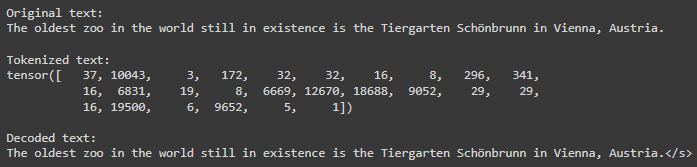
\includegraphics[scale=0.6]{images/tokenization.png}
\caption{Példa a tokenizálásra a T5 modell tokenizálójának használatával.}
\label{fig:tokenization}
\end{figure}

NLP feladatok megoldása során szükségünk lehet arra, hogy a szöveg egyes egységeit megcímkézzük egy adott kategóriával, ezzel segítve a gép számára a megértést. Erre szolgál a \textbf{beszédrész-címkézés}(Part-of-speech tagging). Ennek során a szavakhoz vagy akár az előző feladat alapján generált tokenekhez is hozzárendelhetünk különböző kategóriákat, mégpedig az alapján, hogy az adott egység milyen szerepet tölt be a mondatban. A legelterjedtebb kategóriák közé tartoznak az igék, főnevek, melléknevek, névmások és kötőszavak, de saját egyedi kategóriákkal is elláthatjuk az egységeket.

Bizonyos nyelvek, mint például az angol vagy a magyar tartalmaznak olyan nyelvi elemeket, melyek egy adott feladat megoldása során a gép számára szükségtelenné válhatnak. Ilyen elemek például a ragok. Ezen szükségtelen elemek kiszűrésére és leválasztására szolgál a \textbf{lemmatizáció} és a \textbf{tőképzés}. A lemmatizáció során szavak bizonyos csoportjait(melyeknek általában azonos a szótöve) egyetlen szóban próbálunk meg leírni és a feladatok megoldása során az ezen kategóriájuk szavakhoz ezt az egy szót használjuk majd. A tőképzés folyamatának az eredménye szintén egyetlen szó lesz, azonban ott a konkrét szótő megtalálása lesz a cél és minden azonos szótövű szót erre az egyetlen szótőre cserélünk ki, így könnyítve a gép dolgát. Ezen két módszer arra a feltételezésre épül, hogy az azonos szótövű vagy hasonló kategóriába eső szavak jelentésükben is nagyon közel állnak egymáshoz és ezáltal csökkenthető a különböző szavak darabszáma a szövegben, így gyorsítva a feldolgozást.

Egy újabb feladatkör lehet a szövegfeldolgozás gyorsítására a \textbf{tiltólistás szavak} \\
(stopwords) kiszűrése. Ennek során kiválogatjuk a szövegből azokat a gyakran előforduló szavakat, melyeknek a legkisebb a szemantikai értéke, vagyis amelyek a legkevesebbet adják hozzá a szöveg értelmezéséhez. Ezek lehetnek kötőszavak, névmások, elöljárószavak, de akár tetszőleges, az adott NLP feladat megoldásához számottevően hozzá nem tevő szavak is.

Ahhoz, hogy a gép megfelelően tudjon értelmezni szövegeket elengedhetetlen, hogy a haszontalan szövegelemek mellett a leghasznosabb részeket is ki tudja szűrni. Erre szolgál a \textbf{névelem-felismerés}(Named Entity Recognition), mely feladat során a gépnek ki kell szűrnie bizonyos szavakat vagy mondatrészeket a szövegekből és el kell helyeznie egy adott kategóriában. Ez a kategória lehet városnév, személynév, helynév, cégnév, vagy akár email cím is, attól függően, hogy mire specializáljuk modellünket. Ezen feladat egy komplexebb formája a reláció felismerés, mely annyival bonyolítja meg az alapfeladatot, hogy nem csak egy-egy szót vagy mondatrészt vizsgál, hanem megpróbál kapcsolatokat felfedezni kettő vagy több különböző szó, illetve mondatrész között.

\begin{figure}[h]
\centering
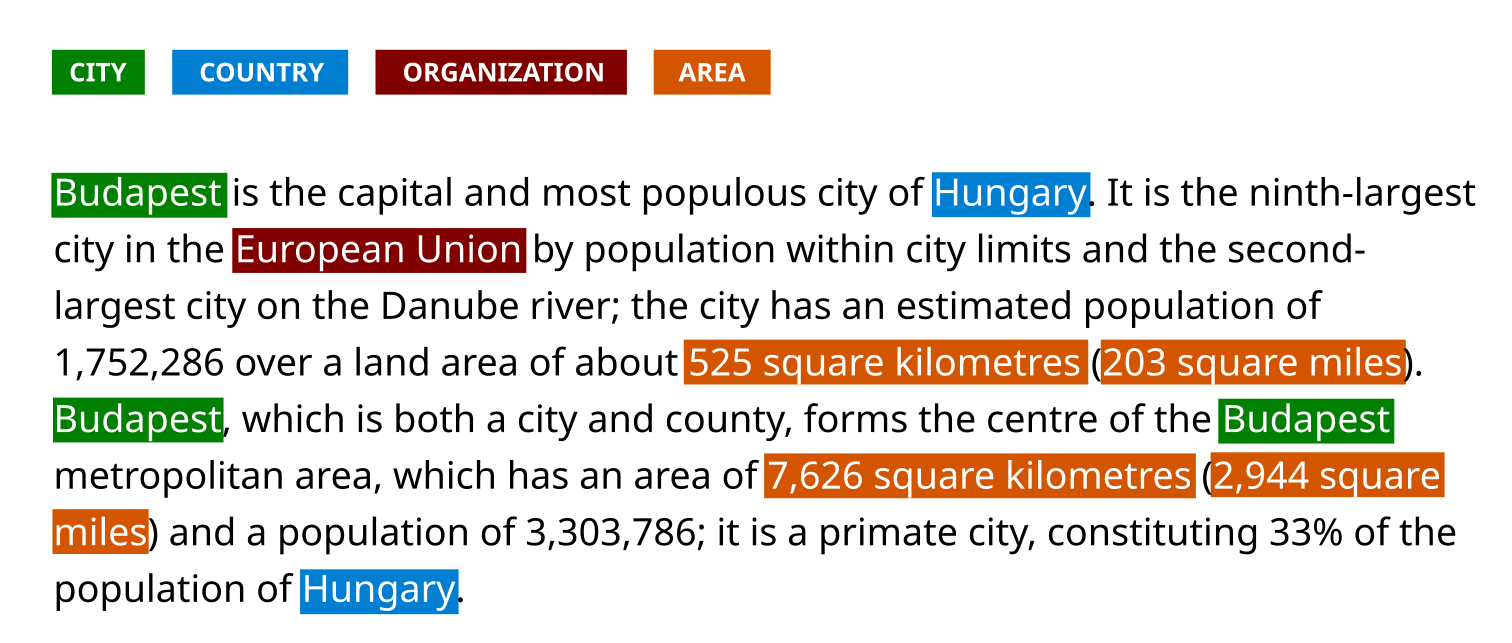
\includegraphics[scale=0.35]{images/named_entity.png}
\caption{Névelem-felismerés a gyakorlatban.}
\label{fig:named_entity}
\end{figure}

Az utóbbi évek talán egyik legnépszerűbb NLP feladatai közé tartozik a \textbf{szövegosztályozás}. A feladat során adottak különböző kategóriák és a gépnek el kell döntenie egy tetszőleges szövegről, hogy mely kategóriába illik. Ennek egyik legelterjedtebb és aktívan használt változata a hangulatelemzés, amikor szövegeket az alapján próbálunk meg kategorizálni, hogy pozitív vagy negatív a hangvételük, vagy hogy milyen egyéb érzelmeket tudnak kiváltani. Erre a feladatra talán a legalkalmasabb megoldások a neurális hálózatok, hiszen ezek alapvetően mintafelismerő rendszerek, így könnyen boldogulnak a feladattal.

	Végezetül elérkeztünk dolgozatom fő NLP témaköréig a \textbf{szöveggeneráláshoz}. Jelenleg talán ez az NLP feladatkör az, ahol a legpopulárisabb eredményeket sikerül elérni az utóbbi időkben, hiszen a ChatGPT megjelenése széles körben elterjesztette az NLP megoldások ezen alkalmazását. Szöveggenerálásnál a gép feladata, hogy egy megadott kontextus alapján hozzon létre szöveget úgy, hogy a kontextus szerepeljen benne, de közben intelligens módon dúsítsa fel vagy éppen csökkentse a kimeneti szöveget valamilyen alfeladatnak megfelelően. A kontextus lehet egy szövegrészlet, egy szó, de akár el is hagyhatjuk és ilyenkor a gép magától alkot egy kontextust és mondjuk egy chatbot esetén beszélgetést kezdeményezhet. A szöveggenerálásnak számos alfeladata van, melyek mind eltérő megközelítést igényelnek, de alapvetően hasonló a céljuk.
	
	Az első alfeladat a \textbf{szövegösszegzés}. Ekkor adott egy bemeneti szöveg és az algoritmusnak szimplán annyi a feladata, hogy kiszűrje belőle a feleslegesnek ítélt részeket és egy rövidebb, tömörebb szöveget adjon vissza eredményül. Ez az alfeladat alkalmas például megbeszélések, előadások rövid összefoglalójának elkészítésére, vagy akár tananyagok alapján tanulási segédanyagok generálására.
	
	Egy újabb alfeladat a \textbf{kérdés megválaszolás}(Question answering). Ekkor a bemeneti kontextus egy kérdés, a kimenet pedig egy vagy több a kérdésre adott válasz. Ezen a területen a legtöbb megoldás természetesen valamilyen adott témakörökben képes csak kérdések megválaszolására, azonban például a ChatGPT, mivel egy majdnem az egész szöveges internetet lefedő adathalmazon lett tanítva, így képes szinte bármilyen témában kérdéseket megválaszolni, akár még formális nyelveken is, például programozási nyelveken vagy a matematika nyelvén.
	
	Az előző alfeladathoz kötődik, de mégis teljesen más kategóriában helyezkedik el dolgozatom fő témája, a \textbf{kérdésgenerálás} feladatköre. Ennél a feladatnál adott nekünk egy szövegrészlet, egy kontextus, amelyhez a gépnek kérdéseket kell alkotnia. A feltehető kérdéseknek több fajtája is van melyeket az alapján csoportosíthatunk, hogy milyen típusú választ várunk rájuk\cite{questions}:

\begin{itemize}
\item Kiegészítendő kérdések
\item Eldöntendő kérdések
\item Választó kérdések
\end{itemize}

Ideális esetben az algoritmus mind a 3 kategóriában képes lesz kérdéseket generálni, de itt is, akár csak a többi esetben a tanítóhalmaz mérete fog majd határt szabni a kontextus témájának és a kérdések típusainak. A kérdésgenerálásnak számos felhasználási területe van, mint például az oktatás, ahol megkönnyítheti a tanárok dolgát dolgozatok készítésekor, vagy akár a hallgatóknak is lehet vele készíteni segédanyagokat. Számos vállalati felhasználása is lehet, mint például felvételi tesztkérdések generálása, de lehet használni ezen megoldásokat akár egy chatbotban is, ahol más NLP feladatokkal együtt fel lehet mérni igényeket vagy beszélgetéseket lehet kezdeményeznie a chatbotnak is. A következő alfejezetben bővebben is kitérek a kérdésgenerálásra, annak módszereivel, típusaival és konkrét felhasználási területeivel együtt.
 
\Section{Kérdésgenerálás}

A kérdésgenerálás feladatköre amellett, hogy hasznos segédeszközök létrehozását segítheti elő, remek mérőeszköze is lehet a mesterséges intelligenciának. Korábban a számítógépekkel történő kommunikáció kimerült abban, hogy különböző parancsokat adtunk a gépnek és azokat igyekezett a lehető legpontosabban elvégezni számunkra. Ez a működés amellett, hogy az ember számára meglehetősen kényelmes, egyben biztosította arról is, hogy akinek a parancsokat megadta, az egy gép és nem ember, hiszen valós, emberi kommunikáció nem történt, hanem csak egy gomb lett megnyomva, egy formális nyelven írt parancs lett megadva vagy egyéb automatika indította el a program futását.

A kérdésgenerálás azonban felbonthatja ezt a korábbi működést és a gépet helyezheti a kérdező pozíciójába. Képzeljünk el például egy ügyfélszolgálati chatbotot, aki felkeres minket valamilyen ügyben és értelmes kérdéseket generálva képes egy adott vállalatnál az ügyfél érdekeit képviselve elvégezni valamilyen adategyeztetési vagy üzleti feladatot. A chatbot ekkor azzal, hogy képes volt adott kontextusban kérdéseket generálni és képes volt az ügyfél által megadott adatokkal kapcsolatban kérdezni egyértelmű tanúbizonyságát adta, hogy intelligens, megértette feladatát és szeretné pontosítani az ügyfél adatait és egyben saját feladatának elvégzését is igyekszik javítani. Ez természetesen még nem jelenti azt, hogy tudatra ébredt a gép, de a felhasználó itt már érezheti azt, hogy intelligens, emberszerű lénnyel beszél.

\SubSection{Kérdésgeneráló alkalmazások}

Magának a feladatnak a formalizálása hosszú időre nyúlik vissza. Az első eredmények a területen a matematikai logika kérdésekre való alkalmazásának idejére tehető. Már 1929-ben \textbf{Cohen} által elkezdődött a kérdések vizsgálata, aki a kérdések tartalmát egy nyitott formulával és egy vagy több kötetlen változóval próbálta leírni\cite{question_generation}, azonban a kérdések automatikus generálása mégis egy még frissnek mondható témakör.

1976-ban \textbf{Wolfe} készített egy tanulást segítő automatikus kérdésgeneráló rendszert AUTOQUEST néven.\cite{autoquest} Itt a kérdések a diákoknak kiadott szöveges anyagokból generálódtak, tehát már itt is körvonalazódott ezen rendszerek alapvető működése. A rendszer képes volt a megadott szövegekből szintaktikai és szemantikai információkat kinyerni. A szöveg szavait háromféle kategóriába sorolta(főnevek, igék és elöljárószavak), melyek segítségével meg tudta határozni a megfelelő kérdő névmást a generált kérdésekhez. A tesztek során a generált kérdések 80\%-a bizonyult helyesnek és értelmesnek, míg szintaktikailag helyesnek a kérdések 93\%-a volt tekinthető.

\textbf{Mostow} és \textbf{Chen} 2009-ben kifejlesztett egy olvasási oktató programot diákoknak, mely automatikus kérdésgenerálást használt, hogy javítsa a tanulók szövegértési képességeit.\cite{reading_tutor} A program alapvető célja, hogy ösztönözze a tanulókat kérdések feltevésére az olvasott szövegekkel kapcsolatban. Ezt úgy éri el, hogy először mutat egy példa kérdést számukra és utána adott választási lehetőségek alapján segít nekik kérdéseket konstruálni az olvasott szövegből. Ha a diák helyes kérdést tett fel, akkor a program pozitív választ ad, míg helytelen esetben új kérdést kell megadni neki. A tesztek során kiderült, hogy a kérdések csupán 35.6\%-a bizonyult helyesnek, azonban a helytelen kérdések detektálásának pontossága 90\% volt, ami nagyon jó eredménynek számított.

A korábbi szöveges kontextus alapú megközelítésekkel szemben 2013-ban \textbf{Jouault} és \textbf{Seta} egy szemantikai alapú kérdésgeneráló programot készített, ami a Wikipedia adatbázisából lekérdezett szemantikai információk alapján képes kérdéseket generálni.\cite{wiki_qg} A felhasználók feladata, hogy egy adott dokumentumból felépítsenek egy idővonalat és felvegyék az egyes események közötti relációkat, tehát egyfajta koncepció vagy szemantikai térképet kell készíteniük. Eközben a program is elkészíti saját koncepciótérképét a felhasználó térképe, illetve a Wikipedia szemantikai információi alapján. Ezt felhasználva a program később kérdéseket tud generálni a felhasználó számára, melyekkel elmélyítheti tudását az adott témában.

\begin{figure}[h]
\centering
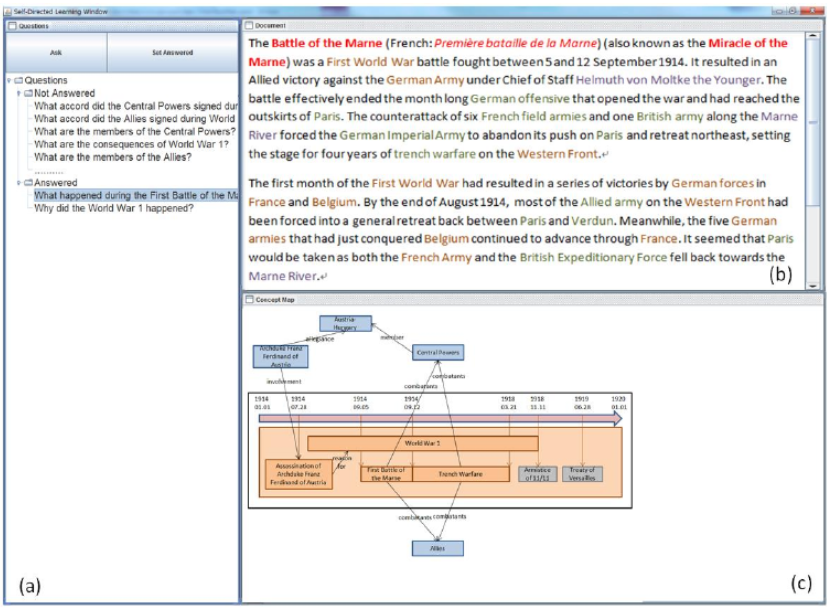
\includegraphics[scale=0.45]{images/wiki_qg.png}
\caption{Jouault és Seta kérdésgeneráló programja.}
\label{fig:wiki_qg}
\end{figure}

\SubSection{Korábbi megközelítések}

Számos megközelítés létezik egy kérdésgenerálási feladat megoldására, azonban ezen megoldásokban több közös lépés is van. Az egyik ilyen lépés az előfeldolgozási fázis, ahol akárcsak a többi NLP feladat esetében a bemenetet a programunk számára kedvező formátumba alakítjuk. Itt lehetőségünk van a szkript számára felesleges szavakat vagy karaktereket kiszűrni és egyszerűsíteni a bemeneten. Egy másik ilyen gyakran ismétlődő lépés, hogy a programnak fel kell tudnia ismernie különböző nyelvtani szerkezeteket, úgy mint főneveket, igéket, névmásokat stb. és ezeket megfelelően csoportosítva értelmeznie kell a mondatot, majd pedig akár ezen kiszűrt lényeges entitások felhasználásával is meg kell konstruálnia az egyes kérdéseket. Utolsó lépésként pedig elő kell állítania a kimenetet általunk is értelmezhető formátumban, természetes vagy formális nyelven, kérdésekként.

Amiben viszont eltérhetnek ezen megoldások, az a közbenső legfőbb lépés, ahol magukat a nyelvtanilag helyes, természetes nyelvű kérdéseket generáljuk.

Az első megközelítés az az \textbf{átalakítás alapú} kérdés generálás. Ennek során az algoritmus először azonosítja és törli az adott célfogalmat a szövegben, megkeresi a megfelelő kérdéstípust és a hozzá tartozó kérdő névmást, majd pedig az igét nyelvtanilag helyes formára alakítja a kiegészítő és modális igék segítségével. Például a \textit{"10 óráig van nyitva a bolt."} mondathoz felismeri az algoritmus az időpontot, leválasztja az időpontra vonatkozó célfogalmat, a kérdés elejére beszúrja a \textit{"Meddig"} kérdő névmást, majd végül már csak át kell alakítania a mondat végi írásjelet és kész is a \textit{"Meddig van nyitva a bolt?"} kérdés. Ez a megközelítés működhet, azonban csak úgy, mint a többi NLP feladat esetén itt is előjön, hogy ha ismeretlen mondattípussal találkozik a rendszer vagy szimplán rosszul megfogalmazott a bemeneti szöveg, esetleg hibás, akkor értelmetlen kérdések fognak generálódni.

Egy másik hasonló megoldás a \textbf{sablon alapú(template-based)} kérdésgenerálás. Itt az az alapötlet, hogy minden kérdéstípushoz létre lehet hozni kontextusspecifikus kérdés sablonokat, melyek a legjobb esetben le fogják fedni az összes kérdésosztályt. Ilyen sablon lehet például a \textit{Mi lenne, ha <X>?} a feltételes módú szövegeknél, vagy a \textit{Mi történik <X>?} és \textit{Mikor lenne <X>?} időbeli kontextusok esetén, ahol az \textit{<X>} változót az algoritmus különböző szemantikai szabályok alapján helyettesíti be. Ez a megoldás elsősorban ismeretközlő szövegek esetében működik, ahol nagyon kötött a szórend és egyértelműen meg lehet találni az egyes változókat. Elbeszélő szövegek esetén szükség lehet egyéb reguláris kifejezés alapú szabályok bevezetésére, melyek segítségével az algoritmus kinyerheti a szükséges információkat a szövegekből. A feladat megközelítése ebben az esetben is eredményes volt, azonban a program feldolgozható témaköreinek növelésével a szükséges szabályhalmaz jelentősen nő és romlik az algoritmus sikeressége is, így ezen megoldásokat leginkább specifikus, zártabb esetekben alkalmazzák.

Napjaink legfejlettebb megoldásai azonban kétségkívül a neurális hálózat alapú mély tanulást alkalmazó algoritmusok. Az ilyen típusú megoldások esetében általánosan elmondható, hogy a fejlesztő nem vesz fel hatalmas méretű szabályhalmazokat a feladat elvégzéséhez, hanem helyette kialakít egy olyan neurális hálózat modellt, mely magától képes ezeket a szabályokat felismerni és ezáltal oldja meg a különböző NLP feladatokat. A következő fejezetben ezen modernebb módszereket fogom bemutatni előnyeikkel és hátrányaikkal együtt.


